% ============================================
% TEMPLATE TUGAS AKHIR POLIWANGI 2023
% Sesuai Pedoman Mutu TA Poliwangi
% ============================================

\documentclass[12pt,a4paper,twoside]{report}

% ============================================
% 1. PACKAGE WAJIB
% ============================================
\usepackage[bahasa]{babel}      % Bahasa Indonesia
\usepackage[utf8]{inputenc}
\usepackage{mathptmx}           % Font Times New Roman (Teks & Math)
\usepackage{geometry}           % Pengaturan Margin
\usepackage{setspace}           % Pengaturan Spasi
\usepackage{graphicx}           % Untuk Gambar
\usepackage[hidelinks]{hyperref}
\usepackage{caption}            % Custom Caption
\usepackage{subcaption}
\usepackage{amsmath}
\usepackage{amssymb}
\usepackage{longtable}
\usepackage{booktabs}
\usepackage{array}
\usepackage{multirow}
\usepackage{titlesec}           % Custom Judul Bab
\usepackage{microtype}
\usepackage{tikz}
\usepackage{float}
\usepackage{graphicx}
\usepackage{pifont}
% Baris di bawah ini SANGAT PENTING, jangan sampai ada yang kurang:
\usetikzlibrary{shapes, arrows, positioning, fit, calc, backgrounds}

% Definisi style (Pastikan ini juga ada)
\tikzset{
    % Style Kotak Biasa
    box/.style={
        rectangle,
        draw=black,
        rounded corners,
        align=center,      % <-- PENTING: Agar bisa pakai enter (\\)
        minimum height=1cm,
        minimum width=2.5cm,
        font=\small
    },
    % Style Input/Output (Jajargenjang/Trapesium)
    io/.style={
        trapezium,
        trapezium left angle=70,
        trapezium right angle=110,
        draw=black,
        fill=white,
        align=center,      % <-- PENTING
        minimum height=1cm,
        minimum width=2.5cm,
        font=\small
    },
    % Style Proses (Persegi Panjang)
    process/.style={
        rectangle,
        draw=black,
        fill=white,
        align=center,      % <-- PENTING
        minimum height=1cm,
        minimum width=2.5cm,
        font=\small
    },
    % Style Decision (Belah Ketupat)
    decision/.style={
        diamond,
        draw=black,
        fill=white,
        align=center,      % <-- PENTING
        aspect=2,
        font=\small
    },
    % Style Group Box (Garis Putus-putus)
    groupbox/.style={
        rectangle,
        draw=black,
        dashed,
        inner sep=0.5cm,
        rounded corners
    },
    % Style Panah
    arrow/.style={
        ->,
        thick,
        >=stealth
    },
    line/.style={
        draw,
        thick
    }
}
% [PENTING] Opsi 'titles' agar judul TOC ikut gaya titlesec (Center)
\usepackage[titles]{tocloft}

\usepackage{apacite}            % Wajib APA Style
\usepackage{indentfirst}        % Indentasi pada paragraf pertama

% ============================================
% 2. PENGATURAN MARGIN (Sesuai Lampiran 1)
% ============================================
\geometry{
    top=2cm,       % ATAS 2 CM
    left=3cm,      % KIRI 3 CM
    right=2cm,     % KANAN 2 CM
    bottom=2cm,    % BAWAH 2 CM
    headheight=15pt
}

% ============================================
% 3. PENGATURAN SPASI & PARAGRAF
% ============================================
\setstretch{1.5}                % Spasi 1.5
\setlength{\parindent}{1.25cm}  % Indentasi baris pertama 1.25 cm
\setlength{\parskip}{0pt}       % Tidak ada spasi tambahan antar paragraf

% ============================================
% 4. PENGATURAN JUDUL BAB (CHAPTER) & SUB-BAB
% ============================================
% Format Judul Bab: 14pt, Bold, Center, Uppercase
\titleformat{\chapter}[display]
    {\normalfont\fontsize{14}{16}\bfseries\centering}
    {\chaptertitlename\ \thechapter}{0pt}{\fontsize{14}{16}\bfseries\uppercase}

% Format Sub-Bab: 12pt, Bold
\titleformat{\section}
    {\normalfont\fontsize{12}{14}\bfseries}
    {\thesection}{1em}{}

\titleformat{\subsection}
    {\normalfont\fontsize{12}{14}\bfseries}
    {\thesubsection}{1em}{}

% Jarak Spasi Judul Bab
\titlespacing*{\chapter}{0pt}{-20pt}{20pt}
\titlespacing*{\section}{0pt}{12pt}{6pt}
\titlespacing*{\subsection}{0pt}{12pt}{6pt}

% ============================================
% 5. PENGATURAN DAFTAR ISI/TABEL/GAMBAR
% ============================================
\renewcommand{\contentsname}{DAFTAR ISI}
\renewcommand{\listfigurename}{DAFTAR GAMBAR}
\renewcommand{\listtablename}{DAFTAR TABEL}
\renewcommand{\bibname}{DAFTAR PUSTAKA}

% Menambahkan titik-titik (leaders) pada Bab di Daftar Isi
\renewcommand{\cftchapleader}{\cftdotfill{\cftdotsep}}

% ============================================
% 6. PENGATURAN CAPTION (TABEL & GAMBAR)
% ============================================
% Tabel: Judul di atas, rata kiri
\captionsetup[table]{
    labelsep=space,
    justification=raggedright,
    singlelinecheck=false,
    position=top,
    font=normalsize
}

% Gambar: Judul di bawah, Center
\captionsetup[figure]{
    labelsep=space,
    justification=centering,
    position=bottom,
    font=normalsize
}

% ============================================
% 7. PENGATURAN NOMOR HALAMAN
% ============================================
\pagestyle{plain} % Bawah Tengah

\newcommand{\frontmatter}{
    \pagenumbering{roman}   % Romawi (i, ii)
    \setcounter{page}{1}
}

\newcommand{\mainmatter}{
    \clearpage
    \pagenumbering{arabic}  % Arab (1, 2)
    \setcounter{page}{1}
}

% ============================================
% 8. IDENTITAS DOKUMEN & VARIABEL
% ============================================
\newcommand{\judulTA}{TRAFFIC ENGINEERING JARINGAN LAYER 2 MENGGUNAKAN GRAPH ATTENTION NETWORK DAN ANALYTIC HIERARCHY PROCESS}
\newcommand{\namaMahasiswa}{AGUNG BAHTIAR}
\newcommand{\nimMahasiswa}{362258302093}
\newcommand{\prodiMahasiswa}{TEKNIK INFORMATIKA}
\newcommand{\tahunPengajuan}{2026}
\newcommand{\pembimbingSatu}{Nama Pembimbing 1, M.T.}
\newcommand{\pembimbingDua}{Nama Pembimbing 2, M.Kom.}

% ============================================
% START DOCUMENT
% ============================================
\begin{document}

% BAGIAN AWAL
\frontmatter
\begin{titlepage}
    \begin{center}
        % --- PENGATURAN JUDUL ---
        \setstretch{1.0}

        % JUDUL TUGAS AKHIR
        % Font 14, Bold, Uppercase, Membentuk Huruf V Terbalik (Piramida Terbalik)
        % Gunakan \\ untuk memenggal kalimat agar baris atas lebih panjang dari bawahnya
        {\fontsize{14}{17}\selectfont \bfseries
        \uppercase{SISTEM REKOMENDASI \textit{TRAFFIC ENGINEERING} JARINGAN\\ \textit{layer} 2 MENGGUNAKAN \textit{GRAPH ATTENTION NETWORK}\\ DAN \textit{ANALYTIC HIERARCHY PROCESS}}
        \par}

        % --- PENGATURAN JARAK VERTIKAL ---

        \setstretch{1.5}

        \vspace{4\baselineskip}

        % --- TIPE DOKUMEN ---
        {\fontsize{12}{14}\selectfont \bfseries PROPOSAL TUGAS AKHIR\par}

        \vspace{2\baselineskip}

        % --- LOGO ---
        \includegraphics[width=4cm, height=4cm]{images/logo-poliwangi.png}\par

        \vspace{5\baselineskip}

        % --- IDENTITAS MAHASISWA ---
        {\setstretch{1.0}
        \fontsize{12}{14}\selectfont \bfseries
        Oleh:\\
        AGUNG BAHTIAR\\
        NIM. 362258302093\par}

        \setstretch{1.5}

        \vspace{6
        \baselineskip}

        % --- INSTITUSI ---
        {\setstretch{1.0}
        \fontsize{16}{19}\selectfont \bfseries
        PROGRAM STUDI SARJANA TERAPAN\\
        TEKNOLOGI REKAYASA PERANGKAT LUNAK\\
        POLITEKNIK NEGERI BANYUWANGI\\
        2026\par}

    \end{center}
\end{titlepage}

\setcounter{page}{2}            % Mulai halaman ii
% % ============================================
% HALAMAN PENGESAHAN
% Sesuai Lampiran 8 Pedoman TA 2023
% ============================================

\chapter*{LEMBAR PENGESAHAN}
\addcontentsline{toc}{chapter}{LEMBAR PENGESAHAN}

% Mengatur posisi vertikal agar muat satu halaman
\vspace*{-1cm}

\begin{center}
    % JUDUL TA [cite: 1021]
    {\fontsize{14}{16}\bfseries\selectfont
    \MakeUppercase{\judulTA}
    \par}

    \vspace{1em}

    % KETERANGAN [cite: 1022-1024]
    {\fontsize{12}{14}\selectfont
    Tugas Akhir disusun untuk Memenuhi Salah Satu Syarat Memperoleh Gelar\\
    % Pilih salah satu sesuai jenjang:
    Sarjana Terapan (S.Tr.)\\
    Politeknik Negeri Banyuwangi
    \par}

    \vspace{1.5em}

    % IDENTITAS MAHASISWA [cite: 1025-1026]
    {\fontsize{12}{14}\selectfont
    \textbf{Oleh:}\\
    \textbf{AGUNG BAHTIAR}\\
    \textbf{NIM. 362258302093}
    \par}

    \vspace{1em}

    % TANGGAL UJIAN [cite: 1027]
    % Ganti tanggal manual atau gunakan command \today
    Tanggal Ujian : ..............................
\end{center}

\vspace{1em}

% BAGIAN TANDA TANGAN PEMBIMBING & PENGUJI
\noindent
\textbf{Menyetujui,}

\vspace{0.5em}

% Menggunakan tabel agar rapi
% Format: Label (Kiri) : Nama (Tengah) Tanda Tangan (Kanan)
\begin{table}[h]
    \centering
    \renewcommand{\arraystretch}{1.5} % Jarak antar baris
    \begin{tabular}{p{3cm} p{0.5cm} p{6cm} l}
        Pembimbing 1 & :  & (.............................) \\
        Pembimbing 2 & :  & (.............................) \\
        Penguji 1    & :  & (.............................) \\
        Penguji 2    & :  & (.............................) \\
    \end{tabular}
\end{table}

\vfill

% BAGIAN PENGESAHAN PEJABAT [cite: 1029-1033]
\begin{center}
    \begin{tabular}{p{6cm} p{1cm} p{6cm}}
        \textbf{Mengesahkan,} & & \textbf{Mengetahui,} \\
        Ketua Jurusan ................. & & Ketua Program Studi \prodiMahasiswa \\

        \vspace{2cm} & & \vspace{2cm} \\ % Ruang Tanda Tangan

        \underline{\textbf{Nama Kajur, Gelar}} & & \underline{\textbf{Nama Kaprodi, Gelar}} \\
        NIK. .............................. & & NIK. .............................. \\
    \end{tabular}
\end{center}

\vfill

\clearpage

% % ============================================
% HALAMAN PERNYATAAN
% ============================================

\chapter*{PERNYATAAN}
\addcontentsline{toc}{chapter}{PERNYATAAN}

\vspace{1cm}

Saya yang bertanda tangan di bawah ini:

\vspace{0.5cm}

\begin{tabular}{lp{0.5cm}l}
Nama & : & \namaMahasiswa \\
NIM & : & \nimMahasiswa \\
\end{tabular}

\vspace{1cm}

Menyatakan dengan sesungguhnya bahwa Tugas Akhir yang berjudul:

\vspace{0.5cm}

\begin{center}
\textbf{``\judulTA''}
\end{center}

\vspace{0.5cm}

adalah benar-benar hasil karya sendiri, kecuali jika disebutkan sumbernya dan belum pernah diajukan pada institusi manapun, serta bukan karya jiplakan/plagiat. Saya bertanggung jawab atas keabsahan dan kebenaran isinya sesuai dengan sikap ilmiah yang harus dijunjung tinggi.

\vspace{0.5cm}

Demikian pernyataan ini saya buat dengan sebenarnya, tanpa adanya tekanan dan paksaan dari pihak manapun serta bersedia mendapat sanksi akademik jika ternyata di kemudian hari pernyataan ini tidak benar.

\vfill

\begin{flushright}
Banyuwangi, \today

\vspace{1.5cm}

Materai 10.000

\vspace{1.5cm}

\namaMahasiswa\\
NIM. \nimMahasiswa
\end{flushright}

\clearpage

% % ============================================
% ABSTRAK BAHASA INDONESIA
% ============================================

\chapter*{ABSTRAK}
\addcontentsline{toc}{chapter}{ABSTRAK}

\begin{center}
    {\fontsize{14}{16}\bfseries\selectfont
    \MakeUppercase{\judulTA}
    \par}

    \vspace{1cm}

    {\fontsize{12}{14}\selectfont
    \namaMahasiswa\\
    NIM. \nimMahasiswa
    \par}

    \vspace{0.5cm}

    {\fontsize{12}{14}\selectfont
    Pembimbing:\\
    1. \pembimbingSatu\\
    2. \pembimbingDua
    \par}
\end{center}

\vspace{1cm}

\setstretch{1.0}
\setlength{\parindent}{1.25cm}

% ISI ABSTRAK (Maksimal 350 kata)
Abstrak berisi ringkasan komprehensif dari seluruh isi Tugas Akhir. Bagian ini mencakup latar belakang singkat yang menjelaskan konteks penelitian, rumusan masalah atau tujuan penelitian, metode penelitian yang digunakan, hasil utama yang diperoleh, dan kesimpulan penting dari penelitian.

Abstrak harus ditulis dalam satu paragraf dengan spasi 1. Hindari penggunaan singkatan yang tidak umum. Jika terpaksa menggunakan singkatan, berikan kepanjangan lengkap pada penggunaan pertama. Abstrak tidak boleh mengandung referensi ke pustaka, tabel, atau gambar.

Untuk penelitian yang bersifat aplikatif atau pembuatan prototype, jelaskan fungsi utama dan keunggulan dari sistem/produk yang dibuat. Untuk penelitian eksperimental, sebutkan variabel-variabel utama yang diteliti dan temuan signifikan yang diperoleh.

Bagian akhir abstrak harus menyebutkan kontribusi utama atau manfaat praktis dari penelitian ini. Total kata dalam abstrak maksimal 350 kata sesuai dengan pedoman Tugas Akhir Poliwangi.

\vspace{1cm}

\noindent\textbf{Kata kunci:} kata kunci 1, kata kunci 2, kata kunci 3, kata kunci 4, kata kunci 5
\\[0.3cm]
\textit{(Maksimal 5 kata kunci, diurutkan alfabetis)}

\setstretch{1.5}
\clearpage

% % ============================================
% ABSTRACT (ENGLISH)
% ============================================

\chapter*{ABSTRACT}
\addcontentsline{toc}{chapter}{ABSTRACT}

\begin{center}
    {\fontsize{14}{16}\bfseries\selectfont
    \MakeUppercase{\judulTA}
    \par}

    \vspace{1cm}

    {\fontsize{12}{14}\selectfont
    \namaMahasiswa\\
    Student ID. \nimMahasiswa
    \par}

    \vspace{0.5cm}

    {\fontsize{12}{14}\selectfont
    Supervisors:\\
    1. \pembimbingSatu\\
    2. \pembimbingDua
    \par}
\end{center}

\vspace{1cm}

\setstretch{1.0}
\setlength{\parindent}{1.25cm}

% ABSTRACT CONTENT (Maximum 350 words)
The abstract contains a comprehensive summary of the entire Final Project. This section includes a brief background explaining the research context, problem formulation or research objectives, research methods used, main results obtained, and important conclusions from the research.

The abstract must be written in one paragraph with single spacing. Avoid using uncommon abbreviations. If it is necessary to use abbreviations, provide the full version at the first use. The abstract should not contain references to literature, tables, or images.

For research that is applicative or prototype making, explain the main functions and advantages of the system/product created. For experimental research, mention the main variables studied and significant findings obtained.

The final part of the abstract should mention the main contribution or practical benefits of this research. The total words in the abstract are a maximum of 350 words according to the Poliwangi Final Project guidelines.

\vspace{1cm}

\noindent\textbf{Keywords:} keyword 1, keyword 2, keyword 3, keyword 4, keyword 5
\\[0.3cm]
\textit{(Maximum 5 keywords, sorted alphabetically)}

\setstretch{1.5}
\clearpage

% % ============================================
% KATA PENGANTAR (VERSI RINGKAS)
% ============================================

\chapter*{KATA PENGANTAR}
\addcontentsline{toc}{chapter}{KATA PENGANTAR}

Puji syukur ke hadirat Tuhan Yang Maha Esa, penulis dapat menyelesaikan Tugas Akhir berjudul ``\textbf{\judulTA}'' ini sebagai syarat memperoleh gelar Sarjana Terapan (S.Tr.) di Program Studi \prodiMahasiswa, Politeknik Negeri Banyuwangi.

Penyusunan laporan ini dapat terlaksana dengan baik berkat dukungan dan bimbingan berbagai pihak. Oleh karena itu, penulis mengucapkan terima kasih kepada:

\begin{enumerate}
    \setlength{\itemsep}{0pt} % Jarak antar poin rapat
    \setlength{\parskip}{0pt}

    \item Direktur Politeknik Negeri Banyuwangi.
    \item Ketua Jurusan Teknik Informatika dan Koordinator Program Studi \prodiMahasiswa.
    \item Bapak/Ibu \pembimbingSatu\ dan \pembimbingDua\ selaku Dosen Pembimbing yang senantiasa memberikan arahan.
    \item Seluruh Dosen dan Staf Politeknik Negeri Banyuwangi.
    \item Kedua orang tua, keluarga, dan rekan-rekan seperjuangan yang selalu memberikan doa dan semangat.
\end{enumerate}

Penulis mengharapkan kritik dan saran yang membangun demi kesempurnaan karya ini. Semoga laporan ini bermanfaat.

\vspace{1.5cm}

\begin{flushright}
    Banyuwangi, \today

    \vspace{2cm} % Ruang Tanda Tangan

    \textbf{\namaMahasiswa}\\
    NIM. \nimMahasiswa
\end{flushright}

\clearpage


% DAFTAR ISI dkk
\clearpage
\addcontentsline{toc}{chapter}{DAFTAR ISI}
\tableofcontents

\clearpage
\addcontentsline{toc}{chapter}{DAFTAR TABEL}
\listoftables

\clearpage
\addcontentsline{toc}{chapter}{DAFTAR GAMBAR}
\listoffigures

% BAGIAN UTAMA
\mainmatter
\chapter{PENDAHULUAN}

\section{Latar Belakang}
PT Lare Osing Ndo merupakan \textit{Internet Service Provider} (ISP) lokal yang beroperasi di Banyuwangi dengan infrastruktur berbasis \textit{switch} Layer 2 dan teknologi VLAN. Pada kondisi saat ini (\textit{current state}), manajemen jaringan komunikasi yang kompleks menghadapi tantangan besar dalam menjaga stabilitas layanan. Pendekatan kecerdasan buatan terdistribusi \cite{alhachem2025} mulai diperlukan untuk menangani tantangan tersebut. Tren pertumbuhan trafik dan pengguna internet berdampak langsung pada ISP regional yang harus menjaga \textit{Service Level Agreement} (SLA). Oleh karena itu, menuju era \textit{zero downtime}, penggunaan \textit{machine learning} menjadi krusial untuk memprediksi kegagalan jaringan sebelum terjadi gangguan fatal \cite{basikolo2023}.

Permasalahan utama muncul pada pengelolaan trafik yang semakin rumit akibat penambahan \textit{link} redundansi yang masif. Saat ini, penentuan jalur masih bergantung pada protokol konvensional atau keputusan manual administrator. Pendekatan ini dinilai kurang efektif karena metode \textit{Traffic Engineering} (TE) modern menuntut kemampuan menangani pola trafik dinamis dan heterogen \cite{marouani2024}, hal yang sulit dicapai oleh algoritma tradisional \cite{jiang2023}. Selain itu, algoritma jalur terpendek konvensional (seperti Dijkstra) membebani \textit{controller} karena harus melakukan kalkulasi ulang secara menyeluruh setiap kali terjadi perubahan topologi sekecil apapun. Akibatnya, sering terjadi ketidakseimbangan beban di mana beberapa jalur mengalami kongesti sementara jalur lain \textit{underutilized}.

Dalam menentukan jalur optimal, terdapat banyak parameter yang perlu dipertimbangkan secara bersamaan, meliputi kinerja perangkat (CPU, RAM) dan kondisi koneksi (kualitas link, \textit{bandwidth}). Setiap parameter memiliki tingkat kepentingan yang berbeda menurut kebijakan ISP. Penentuan bobot prioritas antar parameter ini memerlukan metode pengambilan keputusan multikriteria yang sistematis. \textit{Analytic Hierarchy Process} (AHP) telah terbukti efektif dalam menangani masalah pengambilan keputusan dengan banyak kriteria \cite{saaty2008}, terutama dalam konteks manajemen prioritas jaringan \cite{giouroukelis2026}.

Untuk mengatasi permasalahan ketidakefektifan algoritma konvensional dan subjektivitas parameter tersebut, penelitian ini mengusulkan penerapan metode \textit{Graph Attention Network} (GAT) yang diperkuat dengan pembobotan AHP. \textit{Graph Neural Networks} (GNN) telah terbukti sebagai metode yang \textit{state-of-the-art} untuk menangani data berbentuk graf \cite{wu2021}, yang sangat relevan dengan struktur topologi jaringan \cite{zhou2020}. Secara spesifik, GAT dipilih karena memiliki mekanisme \textit{attention} yang mampu memberikan bobot berbeda pada setiap tetangga \textit{node} \cite{velickovic2017}. Kemampuan ini membuat GAT lebih unggul dibandingkan metode graf konvensional dalam mengenali fitur-fitur penting pada jalur jaringan \cite{kato2024}. Keunggulan utama pendekatan ini adalah kecepatan inferensi secara \textit{real-time} tanpa komputasi iteratif yang berat.

Meskipun integrasi GNN dengan optimasi \textit{routing} mampu meningkatkan ketahanan (\textit{robustness}) jaringan \cite{ye2025}, tantangan utama dalam penerapan AI adalah validitas data latih agar sesuai dengan preferensi operasional. Oleh karena itu, integrasi AHP dalam penelitian ini berfungsi untuk menghasilkan label kualitas jalur yang valid berdasarkan penilaian pakar \cite{khan2020}. Pendekatan hibrida ini diharapkan mampu mempelajari pola aliran trafik secara lebih akurat dibandingkan metode statistik biasa \cite{rahman2023, lassen2025}, sekaligus menutup celah kesenjangan antara kalkulasi matematis murni dengan intuisi operasional pakar jaringan.

\section{Perumusan Masalah}
Berdasarkan latar belakang yang telah diuraikan, maka rumusan masalah dalam penelitian ini adalah:
\begin{enumerate}
    \item Bagaimana menerapkan metode \textit{Analytic Hierarchy Process} (AHP) untuk pembobotan parameter kualitas jaringan (kualitas link, bandwidth, kecepatan, jarak, trafik, CPU, dan RAM) sebagai dasar pembentukan label kualitas jalur?
    \item Bagaimana merancang dan mengimplementasikan arsitektur \textit{Graph Attention Network} (GAT) yang mampu mempelajari representasi graf topologi jaringan dan menghasilkan rekomendasi rute optimal?
    \item Bagaimana performa model GAT dengan pembobotan AHP dalam merekomendasikan jalur dibandingkan dengan metode \textit{shortest path} konvensional berdasarkan metrik akurasi, presisi rekomendasi, dan waktu inferensi?
\end{enumerate}

\section{Tujuan Penelitian}
Tujuan dari penelitian ini adalah untuk:
\begin{enumerate}
    \item Mengimplementasikan metode AHP untuk menghasilkan bobot prioritas parameter jaringan yang valid dan konsisten berdasarkan penilaian pakar, yang kemudian digunakan untuk menghitung skor kualitas jalur sebagai label target dalam pelatihan model.
    \item Membangun dan melatih model rekomendasi rute menggunakan arsitektur GAT dengan konfigurasi optimal dan mekanisme \textit{multi-head attention}, yang mampu mempelajari representasi graf topologi jaringan PT Lare Osing Ndo \cite{velickovic2017}.
    \item Mengevaluasi performa model GAT dalam memprediksi jalur optimal dengan mengukur tingkat akurasi prediksi serta membandingkan skor kualitas jalur yang dihasilkan dengan metode konvensional \cite{almasan2022}.
\end{enumerate}

\section{Manfaat Penelitian}
Manfaat yang diharapkan dari penelitian ini adalah:
\begin{enumerate}
    \item \textbf{Bagi Perusahaan:} Memberikan solusi untuk mempercepat penanganan gangguan dan optimasi trafik menggunakan sistem berbasis kecerdasan buatan, serta menyediakan landasan untuk implementasi otomatisasi jaringan di masa depan.
    \item \textbf{Bagi Akademisi:} Memberikan kontribusi ilmiah terkait penerapan algoritma GAT pada manajemen jaringan WAN/ISP lokal, serta memperkaya studi sebelumnya yang lebih banyak berfokus pada simulasi atau jaringan skala besar \cite{marouani2024, saha2024}.
\end{enumerate}

\section{Batasan Masalah}
Agar penelitian lebih terarah dan fokus pada tujuan utama, batasan masalah yang ditetapkan adalah:
\begin{enumerate}
    \item Data topologi dan parameter jaringan diambil dari perangkat aktif milik PT Lare Osing Ndo, yang terdiri dari atribut \textit{Node} (CPU, RAM, Trafik, Utilisasi) dan atribut \textit{Edge} (Kualitas Link, Bandwidth, Kecepatan, Jarak, Status).
    \item Pembobotan prioritas parameter dilakukan menggunakan metode AHP berdasarkan penilaian pakar (\textit{expert judgment}) dari \textit{network engineer} senior PT Lare Osing Ndo.
    \item Model rekomendasi jalur dibangun menggunakan arsitektur \textit{Graph Attention Network} (GAT) dengan konfigurasi \textit{hyperparameter} (seperti jumlah \textit{layer} dan \textit{hidden units}) yang ditentukan melalui proses eksperimen untuk mendapatkan performa terbaik \cite{fey2019}.
    \item Dataset pelatihan terdiri dari sampel jalur optimal dan sub-optimal dengan proporsi yang disesuaikan untuk kebutuhan pembelajaran model (\textit{supervised learning}).
    \item Pelatihan model dilakukan menggunakan mekanisme \textit{early stopping} untuk menghentikan proses pelatihan secara otomatis ketika model telah mencapai konvergensi optimal.
    \item Evaluasi model difokuskan pada ketepatan prediksi skor kualitas jalur (menggunakan metrik seperti MSE) dan akurasi rekomendasi jalur (\textit{Top-k Precision}) dibandingkan dengan metode konvensional.
    \item Sistem yang dibangun berfokus pada memberikan rekomendasi \textit{top-k} jalur terbaik ($k=3$), dan tidak melakukan konfigurasi otomatis (\textit{auto-configuration}) pada perangkat jaringan.
    \item Pengujian ketahanan model dilakukan melalui simulasi skenario kegagalan tautan (\textit{link failure}) dinamis untuk menguji kemampuan adaptasi model (\textit{inductive learning}) terhadap perubahan topologi.
\end{enumerate}

\chapter{TINJAUAN PUSTAKA}

\section{Landasan Teori}

\subsection{Traffic Engineering}
\textit{Traffic Engineering} (TE) adalah disiplin rekayasa jaringan yang berfokus pada pengukuran, pemodelan, karakterisasi, dan kontrol lalu lintas internet untuk mengoptimalkan kinerja jaringan. Tujuan utama TE adalah meminimalkan kongesti dan meningkatkan pemanfaatan sumber daya melalui penyeimbangan beban trafik (\textit{load balancing}) \cite{marouani2024}.

TE modern membutuhkan kemampuan untuk menangani pola trafik yang dinamis dan beragam, di mana pendekatan konvensional berbasis algoritma statis seperti jalur terpendek (Dijkstra) seringkali tidak mampu beradaptasi dengan kondisi jaringan yang berubah secara real-time. Oleh karena itu, pendekatan berbasis kecerdasan buatan semakin diperlukan untuk melakukan optimasi distribusi trafik secara adaptif dan efisien.

\begin{figure}[H]
    \centering
    \includegraphics[width=0.8\textwidth]{images/te.png}
    \caption{Ilustrasi Traffic Engineering dalam Jaringan}
    \label{fig:traffic_engineering}
\end{figure}

\subsection{Jaringan Layer 2 dan VLAN}
Jaringan Layer 2 beroperasi pada lapisan \textit{Data Link} dalam model OSI, di mana perangkat \textit{switch} mengirimkan frame berdasarkan alamat MAC\@. Teknologi VLAN (\textit{Virtual Local Area Network}) memungkinkan segmentasi jaringan secara logis dalam satu infrastruktur fisik, meningkatkan keamanan dan efisiensi manajemen jaringan. Segmentasi VLAN terbukti dapat meningkatkan performa jaringan dengan membagi \textit{broadcast domain} yang besar menjadi domain-domain yang lebih kecil dan terkelola \cite{warse2025vlan}.

Pada lingkungan ISP yang menggunakan infrastruktur \textit{switching} Layer 2 dengan VLAN, penerapan Traffic Engineering menghadapi tantangan khusus. Mekanisme \textit{Spanning Tree Protocol} (STP) pada Layer 2 cenderung memblokir jalur redundan untuk mencegah \textit{looping}, yang mengakibatkan tautan cadangan tidak termanfaatkan (\textit{underutilized}) \cite{rashid2024performance, aruba2025campus}. Meskipun varian yang lebih modern seperti \textit{Rapid Spanning Tree Protocol} (RSTP) menawarkan konvergensi yang lebih cepat, kondisi ini tetap membuat optimasi jalur menjadi lebih kompleks dibandingkan jaringan IP tradisional (Layer 3) \cite{ahmad2020intervlan}. Oleh karena itu, diperlukan pendekatan cerdas untuk memprediksi kegagalan dan mendistribusikan trafik secara dinamis tanpa melanggar topologi logis Layer 2 \cite{alhachem2025}.

\begin{figure}[H]
    \centering
    % \includegraphics[width=0.8\textwidth]{images/layer2_vlan.png}
    \caption{Arsitektur Jaringan Layer 2 dengan VLAN}
    \label{fig:layer2_vlan}
\end{figure}

\subsection{Kriteria Evaluasi Kualitas Jalur}

Dalam penelitian ini, kualitas jalur jaringan dievaluasi berdasarkan dua kategori utama kriteria: kriteria tingkat node dan kriteria tingkat edge. Pendekatan dual-level ini memastikan evaluasi yang komprehensif dengan mempertimbangkan baik kemampuan perangkat maupun kualitas koneksi \cite{joint_node_edge_optimization, holistic_network_metrics}.

\subsubsection{Kriteria Tingkat Node}

Kriteria tingkat node mengevaluasi kapasitas dan kondisi operasional dari perangkat jaringan (switch/router) yang dilalui oleh sebuah jalur. Berdasarkan literatur resource-aware routing \cite{resource_aware_sdn, node_capacity_routing}, terdapat 6 kriteria yang dipilih:

\begin{enumerate}
    \item \textbf{CPU Score}: Normalized CPU utilization yang menunjukkan ketersediaan processing power \cite{cpu_aware_routing}.
    \item \textbf{RAM Score}: Normalized memory availability untuk buffering dan state management \cite{node_capacity_routing}.
    \item \textbf{Traffic In}: Volume trafik masuk yang sedang ditangani node \cite{utilization_based_te}.
    \item \textbf{Traffic Out}: Volume trafik keluar yang sedang ditangani node \cite{adaptive_utilization_routing}.
    \item \textbf{Utilization Score}: Aggregate interface utilization yang menunjukkan seberapa sibuk node dalam menangani trafik secara keseluruhan \cite{interface_speed_impact}.
    \item \textbf{Status Score}: Binary indicator operational status (up/down) yang sangat penting untuk failure-aware routing \cite{failure_aware_te}.
\end{enumerate}

Skor komposit node dihitung sebagai weighted sum:
\begin{equation}
    S_{node} = \sum_{i=1}^{6} w_i^{node} \cdot f_i^{node}
\end{equation}
\noindent dengan:
\begin{itemize}[label={}, leftmargin=1.5cm, labelsep=0.5cm, noitemsep]
    \item[$S_{node}$] : Skor komposit kualitas node
    \item[$w_i^{node}$] : Bobot prioritas kriteria node ke-$i$ (dari AHP)
    \item[$f_i^{node}$] : Nilai fitur node ke-$i$ yang telah dinormalisasi
\end{itemize}

\subsubsection{Kriteria Tingkat Edge}

Kriteria tingkat edge mengevaluasi karakteristik koneksi fisik atau logis antar perangkat. Mengikuti framework multi-constraint routing \cite{te_multiconstraint}, kriteria yang dipilih meliputi:

\begin{enumerate}
    \item \textbf{Optical Link Quality Score}: Kualitas sinyal optik (OSNR, dBm) pada fiber optic infrastructure \cite{optical_signal_quality}.
    \item \textbf{Error Rate Score}: Inverse dari Bit Error Rate (BER) atau Packet Error Rate (PER) \cite{ber_monitoring}.
    \item \textbf{Packet Loss Score}: Persentase paket yang hilang atau dropped selama transmisi \cite{packet_loss_detection}.
    \item \textbf{Bandwidth Utilization}: Rata-rata utilisasi bandwidth pada kedua arah link (bidirectional average) \cite{bandwidth_aware_te}.
    \item \textbf{Interface Speed}: Kapasitas maksimum interface yang menentukan throughput ceiling \cite{interface_speed_impact}.
    \item \textbf{Distance}: Jarak fisik atau logis yang mempengaruhi propagation delay \cite{geographic_routing}.
    \item \textbf{Status}: Link operational state (up/down) \cite{link_state_routing}.
\end{enumerate}

Skor komposit edge dihitung sebagai:
\begin{equation}
    S_{edge} = \sum_{j=1}^{7} w_j^{edge} \cdot g_j^{edge}
\end{equation}
\noindent dengan:
\begin{itemize}[label={}, leftmargin=1.5cm, labelsep=0.5cm, noitemsep]
    \item[$S_{edge}$] : Skor komposit kualitas edge (link)
    \item[$w_j^{edge}$] : Bobot prioritas kriteria edge ke-$j$ (dari AHP)
    \item[$g_j^{edge}$] : Nilai fitur edge ke-$j$ yang telah dinormalisasi
\end{itemize}

\paragraph{Perbedaan Optical Quality, Error Rate, dan Packet Loss}
Ketiga metrik ini saling melengkapi dalam mengevaluasi kualitas koneksi pada layer yang berbeda:

\begin{enumerate}
    \item \textbf{Optical Link Quality} (Physical Layer): Mengukur kualitas sinyal cahaya pada fiber optic sebelum proses decoding. Parameter seperti OSNR (Optical Signal-to-Noise Ratio), received optical power (dBm), Q-factor, dan chromatic dispersion mengindikasikan seberapa baik sinyal optik dapat dibedakan dari noise \cite{optical_signal_quality, osnr_monitoring}. Degradasi optical quality dapat disebabkan oleh attenuasi fiber, dispersion, atau interferensi optik.

    \item \textbf{Error Rate} (Data Link Layer): Mengukur tingkat kesalahan bit atau paket setelah proses photodetection, analog-to-digital conversion, dan forward error correction (FEC). BER atau PER menunjukkan berapa banyak bit/paket yang corrupt setelah decoding \cite{ber_per_optical, ber_monitoring}. Bahkan dengan optical quality yang baik, error rate bisa tinggi jika ada masalah pada transceiver atau proses decoding.

    \item \textbf{Packet Loss Rate} (Network Layer): Mengukur paket yang hilang atau di-drop karena congestion, buffer overflow, atau TTL expiry, bukan karena corruption \cite{packet_loss_detection}. Packet loss dapat terjadi meskipun optical quality baik dan error rate rendah, terutama saat terjadi congestion pada switch/router.
\end{enumerate}

Kombinasi ketiga metrik ini memberikan gambaran holistik tentang health dari sebuah link, dari physical layer hingga network layer \cite{holistic_network_metrics}. Integrasi multiple edge metrics ini mengikuti paradigma multi-criteria path selection yang telah terbukti efektif dalam traffic engineering modern \cite{routing_multiple_optimality, madm_heuristic_routing, te_multiconstraint, sdn_multiconstraint_routing}.

Pendekatan weighted composite scoring yang mengintegrasikan kriteria node dan edge ini telah terbukti efektif dalam various QoS routing scenarios \cite{qos_composite_metric, weighted_composite_routing, madm_heuristic_routing, routing_multiple_optimality}.


\subsection{Analytic Hierarchy Process (AHP)}

\textit{Analytic Hierarchy Process} (AHP) adalah metode pengambilan keputusan multikriteria yang dikembangkan oleh Thomas L. Saaty untuk menangani masalah kompleks dengan berbagai kriteria bertingkat kepentingan berbeda \cite{saaty2008}. Dalam penelitian ini, AHP berfungsi sebagai \textbf{mekanisme penentuan bobot prioritas fitur} berdasarkan penilaian pakar jaringan PT Lare Osing Ndo. Bobot hasil AHP kemudian diintegrasikan ke dalam perhitungan label kualitas jalur sebagai target pelatihan model GAT, memastikan model mempelajari preferensi operasional yang valid \cite{khan2020}.

\subsubsection{Prinsip Dasar AHP}
AHP mengandalkan tiga prinsip fundamental:
\begin{enumerate}
    \item \textbf{Decomposition}: Pemecahan masalah kompleks menjadi struktur hierarki bertingkat yang terdiri dari tujuan utama, kriteria evaluasi, dan sub-kriteria yang terukur.
    \item \textbf{Comparative Judgement}: Penilaian kepentingan relatif antar elemen melalui perbandingan berpasangan (\textit{pairwise comparison}) menggunakan skala Saaty.
    \item \textbf{Logical Consistency}: Verifikasi konsistensi penilaian melalui pengujian Consistency Ratio (CR) untuk memastikan reliabilitas hasil.
\end{enumerate}

\subsubsection{Struktur Hierarki AHP}
Hierarki AHP dalam penelitian ini disusun untuk mengonversi preferensi subjektif manajemen jaringan menjadi bobot kuantitatif. Struktur terdiri dari tiga tingkat seperti diilustrasikan pada Gambar \ref{fig:ahp_hierarchy}. Hasil akhir proses ini adalah dua vektor bobot: $\mathbf{w}_{node} \in \mathbb{R}^6$ dan $\mathbf{w}_{edge} \in \mathbb{R}^7$.

\begin{figure}[H]
    \centering
    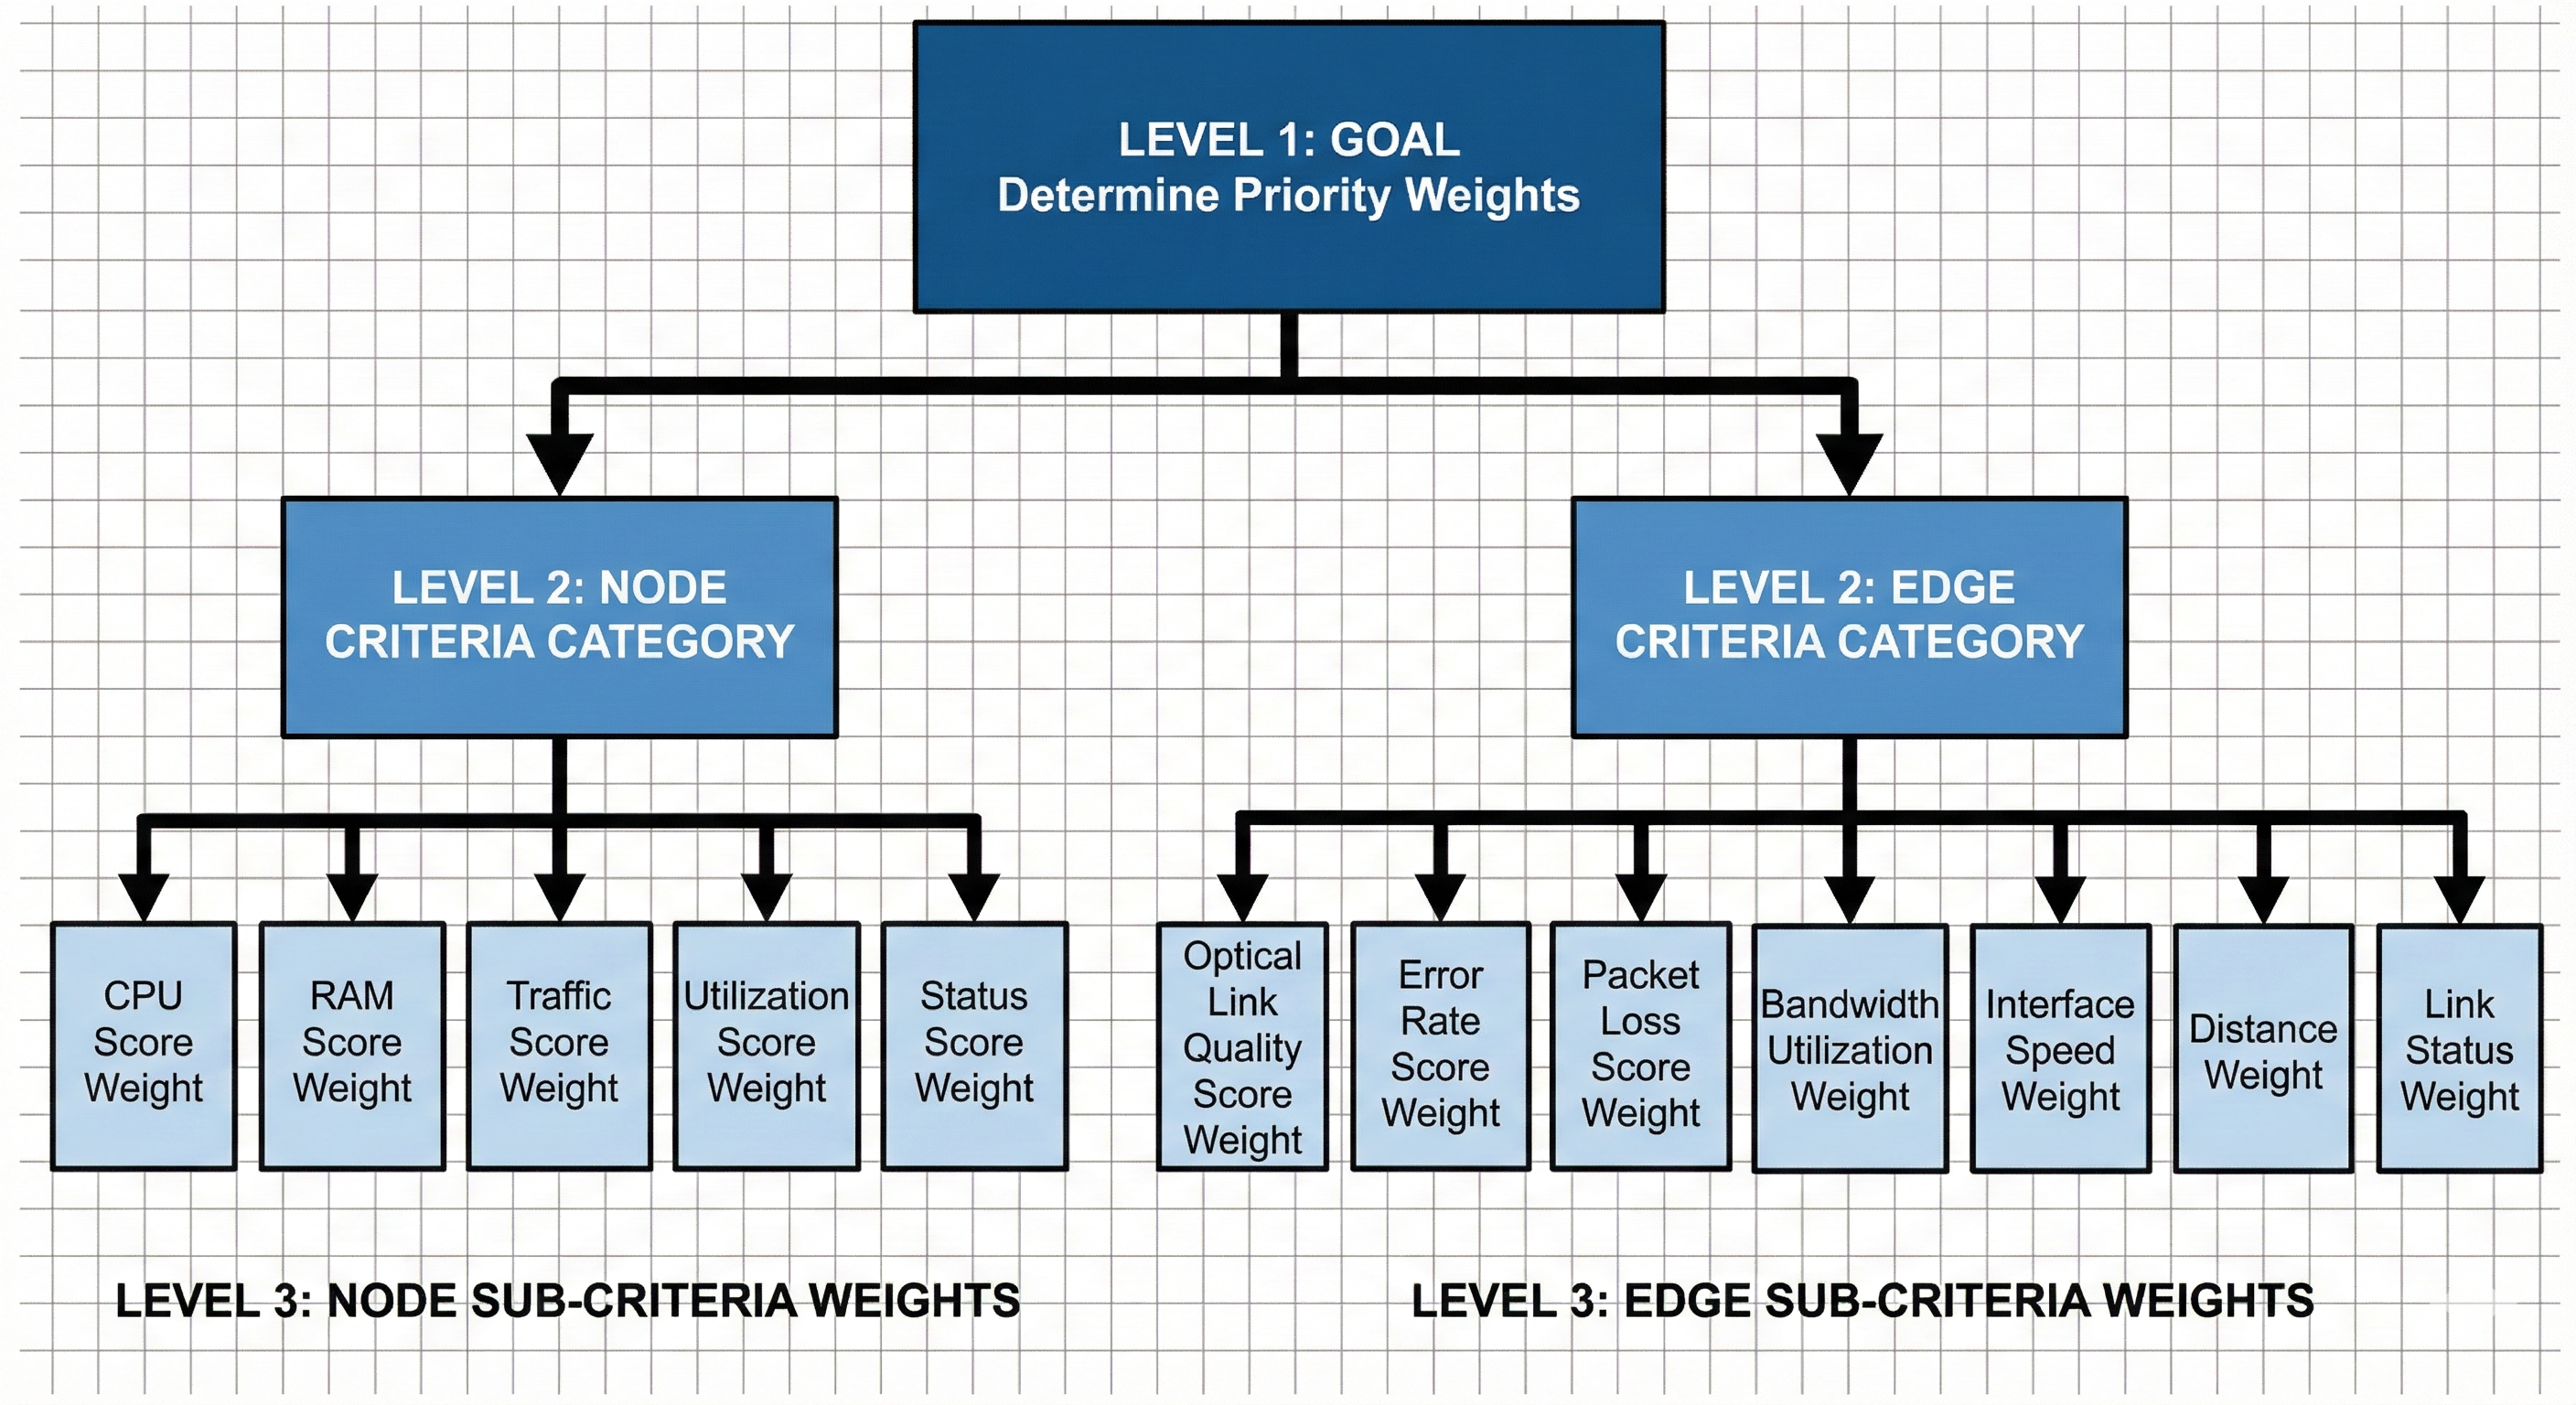
\includegraphics[width=0.9\textwidth]{images/hirarki.png}
    \caption{Struktur Hierarki AHP untuk Penentuan Bobot Parameter}
    \label{fig:ahp_hierarchy}
\end{figure}

\subsubsection{Tahapan Metode AHP}
Implementasi AHP meliputi lima tahapan sistematis yang dijelaskan berikut ini:

\paragraph{1. Penyusunan Matriks Perbandingan Berpasangan}
Matriks perbandingan disusun dengan membandingkan setiap pasangan kriteria berdasarkan skala Saaty. Matriks berukuran $n \times n$ ini bersifat resiprokal:

\begin{equation}
    \mathbf{A} = \begin{bmatrix}
        1 & a_{12} & \cdots & a_{1n} \\
        1/a_{12} & 1 & \cdots & a_{2n} \\
        \vdots & \vdots & \ddots & \vdots \\
        1/a_{1n} & 1/a_{2n} & \cdots & 1
    \end{bmatrix}, \quad a_{ji} = \frac{1}{a_{ij}}
\end{equation}
\noindent dengan:
\begin{itemize}[label={}, leftmargin=1.5cm, labelsep=0.5cm, noitemsep]
    \item[$\mathbf{A}$] : Matriks perbandingan berpasangan AHP
    \item[$a_{ij}$] : Nilai perbandingan kepentingan kriteria $i$ terhadap kriteria $j$
    \item[$n$] : Jumlah kriteria yang dibandingkan
\end{itemize}

Skala penilaian mengikuti standar Saaty seperti ditunjukkan Tabel \ref{tab:saaty_scale}.

\begin{table}[H]
\centering
\caption{Skala Perbandingan Berpasangan Saaty}
\label{tab:saaty_scale}
\begin{tabular}{|c|l|}
\hline
\textbf{Nilai} & \textbf{Interpretasi} \\
\hline
1 & Kedua elemen sama pentingnya \\
3 & Elemen pertama sedikit lebih penting \\
5 & Elemen pertama lebih penting \\
7 & Elemen pertama sangat lebih penting \\
9 & Elemen pertama mutlak lebih penting \\
2, 4, 6, 8 & Nilai antara untuk kompromi \\
\hline
\end{tabular}
\end{table}

\paragraph{2. Normalisasi Matriks Perbandingan}
Setiap kolom matriks dinormalisasi dengan membagi setiap elemen terhadap total kolomnya:

\begin{equation}
    T_j = \sum_{i=1}^{n} a_{ij}, \quad n_{ij} = \frac{a_{ij}}{T_j}
\end{equation}
\noindent dengan:
\begin{itemize}[label={}, leftmargin=1.5cm, labelsep=0.5cm, noitemsep]
    \item[$T_j$] : Total jumlah nilai pada kolom $j$
    \item[$n_{ij}$] : Nilai elemen matriks yang telah dinormalisasi
\end{itemize}

\paragraph{3. Perhitungan Vektor Prioritas dan Bobot}
Vektor prioritas diperoleh dari rata-rata baris matriks ternormalisasi:

\begin{equation}
    PV_i = \sum_{j=1}^{n} n_{ij}, \quad w_i = \frac{PV_i}{n}
\end{equation}
\noindent dengan:
\begin{itemize}[label={}, leftmargin=1.5cm, labelsep=0.5cm, noitemsep]
    \item[$PV_i$] : Nilai prioritas (jumlah baris ternormalisasi)
    \item[$w_i$] : Bobot prioritas akhir untuk kriteria $i$
\end{itemize}

\paragraph{4. Uji Konsistensi}

Langkah pertama dalam uji konsistensi adalah menghitung nilai eigen maksimum ($\lambda_{max}$) yang diperoleh dari rata-rata rasio antara vektor konsistensi ($CV$) dengan bobot prioritas ($w$):

\begin{equation}
    \lambda_{max} = \frac{1}{n} \sum_{i=1}^{n} \frac{CV_i}{w_i}
\end{equation}
\noindent dengan:
\begin{itemize}[label={}, leftmargin=1.5cm, labelsep=0.5cm, noitemsep]
    \item[$\lambda_{max}$] : Nilai eigen maksimum dari matriks perbandingan
    \item[$CV_i$] : Elemen vektor konsistensi baris ke-$i$ (hasil perkalian matriks dengan bobot)
    \item[$w_i$] : Bobot prioritas kriteria ke-$i$
    \item[$n$] : Jumlah kriteria (orde matriks)
\end{itemize}

Selanjutnya, dihitung nilai \textit{Consistency Index} (CI) untuk mengukur penyimpangan konsistensi data:

\begin{equation}
    CI = \frac{\lambda_{max} - n}{n - 1}
\end{equation}
\noindent dengan:
\begin{itemize}[label={}, leftmargin=1.5cm, labelsep=0.5cm, noitemsep]
    \item[$CI$] : \textit{Consistency Index}
    \item[$\lambda_{max}$] : Nilai eigen maksimum
    \item[$n$] : Jumlah elemen atau kriteria yang dibandingkan
\end{itemize}

Terakhir, rasio konsistensi atau \textit{Consistency Ratio} (CR) dihitung dengan membandingkan nilai CI terhadap \textit{Random Index} (RI):

\begin{equation}
    CR = \frac{CI}{RI}
\end{equation}
\noindent dengan:
\begin{itemize}[label={}, leftmargin=1.5cm, labelsep=0.5cm, noitemsep]
    \item[$CR$] : \textit{Consistency Ratio}
    \item[$RI$] : \textit{Random Consistency Index}
\end{itemize}

Nilai referensi untuk \textit{Random Index} (RI) bergantung pada jumlah kriteria ($n$) yang digunakan, seperti yang disajikan pada Tabel \ref{tab:ri_index}.

\begin{table}[H]
\centering
\caption{Nilai Random Index (RI)}
\label{tab:ri_index}
\begin{tabular}{|c|c|c|c|c|c|c|c|c|c|c|}
\hline
\textbf{n} & 1 & 2 & 3 & 4 & 5 & 6 & 7 & 8 & 9 & 10 \\
\hline
\textbf{RI} & 0 & 0 & 0{,}58 & 0{,}90 & 1{,}12 & 1{,}24 & 1{,}32 & 1{,}41 & 1{,}45 & 1{,}49 \\
\hline
\end{tabular}
\end{table}

Suatu matriks perbandingan dinyatakan konsisten dan dapat diterima jika nilai $CR \leq 0{,}1$. Jika nilai $CR > 0{,}1$, maka penilaian perbandingan berpasangan perlu diperbaiki ulang.

\paragraph{5. Output Bobot AHP}
Tahap ini menghasilkan vektor bobot final $\mathbf{w}_{node}$ dan $\mathbf{w}_{edge}$ yang siap diintegrasikan ke dalam perhitungan skor kualitas jalur.

\subsection{Graph Attention Network (GAT)}

\textit{Graph Attention Network} (GAT) merupakan evolusi dari \textit{Graph Neural Networks} (GNN) yang mengintegrasikan mekanisme \textit{masked self-attention} untuk mengatasi keterbatasan pendekatan berbasis graf konvensional \cite{velickovic2017}. GAT memungkinkan model untuk "memfokuskan perhatian" pada jalur dengan kualitas superior dan mengurangi pengaruh jalur yang mengalami degradasi \cite{kato2024}.

\subsubsection{Representasi Graf Jaringan}

Topologi jaringan dimodelkan sebagai graf tidak berarah $\mathcal{G} = (\mathcal{V}, \mathcal{E})$. Setiap node $v_i \in \mathcal{V}$ memiliki vektor fitur $\vec{h}_i$, sementara setiap edge $e_{ij} \in \mathcal{E}$ memiliki atribut $\vec{f}_{ij}$.

\paragraph{Struktur Konektivitas Graf}
Konektivitas antar node direpresentasikan melalui matriks adjacency $\mathbf{A}$. Himpunan tetangga node $i$ didefinisikan sebagai:

\begin{equation}
    \mathcal{N}_i = \{v_j \in \mathcal{V} : A_{ij} = 1\}
\end{equation}
\noindent dengan:
\begin{itemize}[label={}, leftmargin=1.5cm, labelsep=0.5cm, noitemsep]
    \item[$\mathcal{N}_i$] : Himpunan node tetangga yang terhubung langsung ke node $i$
    \item[$A_{ij}$] : Elemen matriks adjacency ($1$ jika terhubung, $0$ jika tidak)
\end{itemize}

\paragraph{Integrasi Fitur Edge dalam GAT}
Penelitian ini mengadopsi strategi \textbf{Edge Feature Concatenation}, dimana fitur edge digabungkan dengan fitur node dalam perhitungan skor attention:

\begin{equation}
    s_{ij} = \text{LeakyReLU}\left(\vec{a}^T [\mathbf{W}\vec{h}_i \, \| \, \mathbf{W}\vec{h}_j \, \| \, \mathbf{W}_e\vec{f}_{ij}]\right)
\end{equation}
\noindent dengan:
\begin{itemize}[label={}, leftmargin=1.5cm, labelsep=0.5cm, noitemsep]
    \item[$s_{ij}$] : Skor attention awal yang melibatkan fitur edge
    \item[$\vec{a}$] : Vektor parameter weight vector untuk mekanisme attention
    \item[$\mathbf{W}, \mathbf{W}_e$] : Matriks transformasi linear untuk fitur node dan edge
    \item[$\vec{h}, \vec{f}$] : Vektor fitur node dan vektor fitur edge
    \item[$\|$] : Operasi concatenation (penggabungan)
\end{itemize}

\subsubsection{Tahapan Komputasi GAT}

\paragraph{1. Transformasi Linear Fitur Input}
Fitur input setiap node ditransformasi ke ruang fitur yang lebih ekspresif:
\begin{equation}
    \vec{z}_i = \mathbf{W} \vec{h}_i
\end{equation}
\noindent dengan:
\begin{itemize}[label={}, leftmargin=1.5cm, labelsep=0.5cm, noitemsep]
    \item[$\vec{z}_i$] : Fitur node $i$ setelah transformasi linear
    \item[$\mathbf{W}$] : Matriks bobot yang dipelajari (learnable weight matrix)
\end{itemize}

\paragraph{2. Komputasi Skor Attention Mentah}
Kepentingan relatif node tetangga $j$ terhadap node $i$ dihitung menggunakan mekanisme attention:
\begin{equation}
    e_{ij} = \text{LeakyReLU}\left(\vec{a}^T [\vec{z}_i \, \| \, \vec{z}_j]\right)
\end{equation}
\noindent dengan:
\begin{itemize}[label={}, leftmargin=1.5cm, labelsep=0.5cm, noitemsep]
    \item[$e_{ij}$] : Koefisien attention mentah (belum dinormalisasi)
\end{itemize}

Fungsi LeakyReLU didefinisikan sebagai:
\begin{equation}
    \text{LeakyReLU}(x) = \begin{cases}
        x & \text{jika } x \geq 0 \\
        \lambda x & \text{jika } x < 0
    \end{cases}
\end{equation}
\noindent dengan:
\begin{itemize}[label={}, leftmargin=1.5cm, labelsep=0.5cm, noitemsep]
    \item[$\lambda$] : Slope untuk nilai negatif (biasanya 0.01 - 0.2)
\end{itemize}

\paragraph{3. Normalisasi dengan Softmax}
Skor attention mentah dinormalisasi menjadi distribusi probabilitas:
\begin{equation}
    \alpha_{ij} = \text{softmax}_j(e_{ij}) = \frac{\exp(e_{ij})}{\sum_{k \in \mathcal{N}_i \cup \{i\}} \exp(e_{ik})}
\end{equation}
\noindent dengan:
\begin{itemize}[label={}, leftmargin=1.5cm, labelsep=0.5cm, noitemsep]
    \item[$\alpha_{ij}$] : Koefisien attention ternormalisasi (tingkat kepentingan node $j$ bagi $i$)
\end{itemize}

\paragraph{4. Agregasi Fitur dengan Weighted Sum}
Informasi dari node tetangga diagregasi menggunakan weighted sum:
\begin{equation}
    \vec{h'}_i = \sigma\left(\sum_{j \in \mathcal{N}_i \cup \{i\}} \alpha_{ij} \vec{z}_j\right)
\end{equation}
\noindent dengan:
\begin{itemize}[label={}, leftmargin=1.5cm, labelsep=0.5cm, noitemsep]
    \item[$\vec{h'}_i$] : Fitur output node $i$
    \item[$\sigma$] : Fungsi aktivasi non-linear (misalnya ELU)
\end{itemize}

\paragraph{5. Multi-Head Attention}
Output dari $K$ heads digabungkan melalui concatenation:
\begin{equation}
    \vec{h'}_i = \Bigg\|_{k=1}^{K} \sigma\left(\sum_{j \in \mathcal{N}_i \cup \{i\}} \alpha_{ij}^k \mathbf{W}^k\vec{h}_j\right)
\end{equation}

Untuk output layer (prediksi final), digunakan averaging:
\begin{equation}
    \vec{h'}_i = \sigma\left(\frac{1}{K}\sum_{k=1}^{K} \sum_{j \in \mathcal{N}_i \cup \{i\}} \alpha_{ij}^k \mathbf{W}^k\vec{h}_j\right)
\end{equation}
\noindent dengan:
\begin{itemize}[label={}, leftmargin=1.5cm, labelsep=0.5cm, noitemsep]
    \item[$K$] : Jumlah attention heads yang berjalan paralel
    \item[$\alpha_{ij}^k$] : Koefisien attention pada head ke-$k$
\end{itemize}

\subsection{Integrasi AHP dengan GAT}

Penelitian ini mengintegrasikan AHP dengan GAT melalui mekanisme \textit{Expert-Guided Feature Weighting}.

\subsubsection{Perhitungan Skor Kualitas Node dan Edge}
Skor kualitas setiap komponen jaringan dihitung menggunakan weighted sum:

\begin{equation}
    Q_{node}(v) = \sum_{k=1}^{6} w_k^{node} \cdot s_k(v)
\end{equation}

\begin{equation}
    Q_{edge}(e) = \sum_{k=1}^{7} w_k^{edge} \cdot s_k(e)
\end{equation}
\noindent dengan:
\begin{itemize}[label={}, leftmargin=1.5cm, labelsep=0.5cm, noitemsep]
    \item[$Q_{node}(v)$] : Skor kualitas node $v$
    \item[$Q_{edge}(e)$] : Skor kualitas edge $e$
    \item[$s_k$] : Nilai parameter ke-$k$ yang telah dinormalisasi
\end{itemize}

\subsubsection{Perhitungan Skor Kualitas Jalur}
Skor kualitas jalur secara keseluruhan dihitung dengan pendekatan weighted average yang dimodifikasi dengan penalti hop:

\begin{equation}
    Q_{path} = \left( \frac{\sum_{v \in P} Q_{node}(v) + \sum_{e \in P} Q_{edge}(e)}{|P|_{components}} \right) \times (1 - \text{Penalty}_{hop})
\end{equation}
\noindent dengan:
\begin{itemize}[label={}, leftmargin=1.5cm, labelsep=0.5cm, noitemsep]
    \item[$Q_{path}$] : Skor kualitas jalur keseluruhan
    \item[$P$] : Himpunan node dan edge dalam jalur
    \item[$|P|_{components}$] : Jumlah total komponen (node + edge) dalam jalur
\end{itemize}

Penalti hop didefinisikan sebagai:
\begin{equation}
    \text{Penalty}_{hop} = \alpha \cdot \frac{h}{h_{max}}
\end{equation}
\noindent dengan:
\begin{itemize}[label={}, leftmargin=1.5cm, labelsep=0.5cm, noitemsep]
    \item[$\alpha$] : Koefisien sensitivitas penalti
    \item[$h$] : Jumlah hop pada jalur saat ini
    \item[$h_{max}$] : Jumlah hop maksimum dalam topologi jaringan
\end{itemize}

\subsubsection{Alur Kerja Integrasi AHP-GAT}
Gambar \ref{fig:ahp_gat_integration} mengilustrasikan alur kerja lengkap integrasi AHP dengan GAT.

\begin{figure}[H]
    \centering
    \resizebox{0.95\textwidth}{!}{%
    \begin{tikzpicture}[
        node distance=1.2cm and 1.5cm,
        box/.style={
            rectangle,
            rounded corners,
            draw=black!70,
            minimum width=3.5cm,
            minimum height=1cm,
            align=center,
            font=\small,
            fill=white,
            drop shadow
        },
        databox/.style={
            box,
            fill=blue!10
        },
        processbox/.style={
            box,
            fill=green!10
        },
        resultbox/.style={
            box,
            fill=orange!10
        },
        arrow/.style={
            ->,
            thick,
            >=stealth,
            color=black!70
        },
        labelstyle/.style={
            font=\bfseries\small,
            align=center
        }
    ]

    % ===== STAGE 1: EXPERT WEIGHTING =====
    \node[processbox] (expert) {Expert\\Judgment};
    \node[processbox, below=of expert] (ahp) {\textbf{AHP Process}\\Pairwise Comparison\\Consistency Check};
    \node[databox, below=of ahp] (weights) {Weight Vectors\\$\mathbf{w}_{node} \in \mathbb{R}^6$\\$\mathbf{w}_{edge} \in \mathbb{R}^7$};

    % ===== STAGE 2: RULE-BASED LABELING =====
    \node[databox, right=2cm of expert] (features) {Network Metrics\\Node Features\\Edge Features};
    \node[processbox, below=of features] (scoring) {\textbf{Rule-Based Scoring}\\Weighted Sum\\Hop Penalty};
    \node[databox, below=of scoring] (labels) {Ground Truth\\$Q_{path}$ Labels\\(Target Values)};

    % ===== STAGE 3: GAT TRAINING =====
    \node[processbox, right=2cm of features] (gat) {\textbf{GAT Training}\\Multi-Head Attention\\Graph Convolution\\MSE Loss};
    \node[resultbox, below=of gat] (model) {Trained Model\\Path Quality\\Predictor};

    % ===== STAGE 4: INFERENCE =====
    \node[databox, right=1.5cm of gat] (newdata) {New Network\\State\\(Real-time)};
    \node[resultbox, below=of newdata] (prediction) {Path Quality\\Prediction\\$\hat{Q}_{path}$};

    % ===== ARROWS STAGE 1 =====
    \draw[arrow] (expert) -- (ahp) node[midway, right, font=\scriptsize] {preferences};
    \draw[arrow] (ahp) -- (weights) node[midway, right, font=\scriptsize] {validated};

    % ===== ARROWS STAGE 2 =====
    \draw[arrow] (weights) -- (scoring) node[midway, above, font=\scriptsize] {apply};
    \draw[arrow] (features) -- (scoring) node[midway, right, font=\scriptsize] {input};
    \draw[arrow] (scoring) -- (labels) node[midway, right, font=\scriptsize] {compute};

    % ===== ARROWS STAGE 3 =====
    \draw[arrow] (features) -- (gat) node[midway, above, font=\scriptsize] {features};
    \draw[arrow] (labels) -- (gat) node[midway, above, font=\scriptsize] {targets};
    \draw[arrow] (gat) -- (model) node[midway, right, font=\scriptsize] {optimize};

    % ===== ARROWS STAGE 4 =====
    \draw[arrow] (model) -- (prediction) node[midway, above, font=\scriptsize] {inference};
    \draw[arrow] (newdata) -- (prediction) node[midway, right, font=\scriptsize] {input};

    % ===== STAGE LABELS =====
    \node[labelstyle, above=0.4cm of expert] {Stage 1\\Expert Weighting};
    \node[labelstyle, above=0.4cm of features] {Stage 2\\Rule-Based Labeling};
    \node[labelstyle, above=0.4cm of gat] {Stage 3\\Supervised Learning};
    \node[labelstyle, above=0.4cm of newdata] {Stage 4\\Real-time Inference};

    % ===== DASHED GROUPING BOXES =====
    \node[draw=blue!50, dashed, rounded corners, fit=(expert)(ahp)(weights),
          inner sep=0.3cm, label={[anchor=south, font=\scriptsize]below:AHP Module}] {};
    \node[draw=green!50, dashed, rounded corners, fit=(features)(scoring)(labels),
          inner sep=0.3cm, label={[anchor=south, font=\scriptsize]below:Labeling Module}] {};
    \node[draw=orange!50, dashed, rounded corners, fit=(gat)(model),
          inner sep=0.3cm, label={[anchor=south, font=\scriptsize]below:Learning Module}] {};
    \node[draw=red!50, dashed, rounded corners, fit=(newdata)(prediction),
          inner sep=0.3cm, label={[anchor=south, font=\scriptsize]below:Deployment Module}] {};

    \end{tikzpicture}%
    }
    \caption{Alur Integrasi AHP dengan GAT dalam Sistem Rekomendasi Jalur}
    \label{fig:ahp_gat_integration}
\end{figure}

Penjelasan detail setiap tahapan adalah sebagai berikut:

\begin{enumerate}
    \item \textbf{Stage 1 - Expert Weighting}: Pakar jaringan melakukan penilaian AHP untuk menghasilkan vektor bobot $\mathbf{w}_{node}$ dan $\mathbf{w}_{edge}$.
    \item \textbf{Stage 2 - Rule-Based Labeling}: Sistem menghitung skor $Q_{path}$ sebagai ground truth sintetis.
    \item \textbf{Stage 3 - Supervised Learning}: Model GAT dilatih untuk meminimalkan loss Mean Squared Error (MSE):
        \begin{equation}
            \mathcal{L} = \frac{1}{N} \sum_{i=1}^{N} \left(Q_{pred}^{(i)} - Q_{target}^{(i)}\right)^2
        \end{equation}
        \noindent dengan:
        \begin{itemize}[label={}, leftmargin=1.5cm, labelsep=0.5cm, noitemsep]
            \item[$\mathcal{L}$] : Nilai Loss Function (MSE)
            \item[$N$] : Jumlah sampel data training
            \item[$Q_{pred}$] : Prediksi kualitas jalur dari model GAT
            \item[$Q_{target}$] : Label kualitas jalur (Ground Truth) dari Stage 2
        \end{itemize}
    \item \textbf{Stage 4 - Real-time Inference}: Model memprediksi kualitas jalur $\hat{Q}_{path}$ secara real-time.
\end{enumerate}

\section{Penelitian Terkait}
% (Bagian ini tetap sama seperti sebelumnya, tidak ada perubahan rumus)
Tinjauan studi dilakukan untuk memetakan posisi penelitian ini terhadap penelitian-penelitian sebelumnya yang relevan... (Lanjutan teks asli Anda)

\begin{table}[ht]
    \centering
    \caption{State of the Art Penelitian}
    \label{tab:state_of_the_art}
    \small
    \begin{tabular}{p{3cm} p{3cm} p{2.5cm} p{4.5cm}}
        \hline
        \textbf{Peneliti (Tahun)} & \textbf{Masalah} & \textbf{Metode} & \textbf{Hasil \& Perbedaan} \\
        \hline
        \cite{marouani2024} & Optimasi trafik pada WAN & GAT & Unggul di topologi dinamis. \textbf{Bedanya:} Penelitian ini menambahkan validasi pakar via AHP. \\
        \hline
       \cite{almasan2022} & Optimasi \textit{Routing} & DRL + GNN & Generalisasi baik tapi training berat. \textbf{Bedanya:} Penelitian ini menggunakan \textit{Supervised Learning} yang lebih efisien. \\
        \hline
        \cite{rahman2023} & Prediksi Trafik & GCN & Efektif spasial. \textbf{Bedanya:} GAT memiliki mekanisme \textit{attention} yang lebih presisi dibanding GCN. \\
        \hline
        \textbf{Penelitian Ini} & \textbf{Rekomendasi Jalur ISP} & \textbf{GAT + AHP} & \textbf{Integrasi \textit{expert judgment} (AHP) ke dalam arsitektur \textit{Deep Learning} (GAT).} \\
        \hline
    \end{tabular}
\end{table}

\section{Kerangka Pemikiran}
% (Bagian ini tetap sama seperti sebelumnya)
Kerangka pemikiran menggambarkan alur logika penelitian dari variabel yang diobservasi hingga pengukuran keberhasilan... (Lanjutan teks asli Anda)

\begin{figure}[ht]
    \centering
    \resizebox{\textwidth}{!}{%
    \begin{tikzpicture}[
        node distance=0.6cm and 0.8cm, % Jarak Vertikal dan Horizontal
        box/.style={
            rectangle,
            draw=black!70,
            rounded corners,
            minimum width=3.5cm,
            minimum height=1cm,
            align=center,
            font=\small,
            fill=white,
            drop shadow
        },
        header/.style={
            font=\bfseries\large,
            align=center
        },
        groupbox/.style={
            draw=black!50,
            rounded corners,
            dashed,
            inner sep=0.4cm,
            align=center
        },
        arrow/.style={
            ->,
            thick,
            >=stealth,
            color=black!80
        }
    ]

    % --- COLUMN 1: INDICATORS ---
    \node[header] (ind_title) {INDICATORS};
    \node[box, below=0.5cm of ind_title] (cpu) {CPU \& RAM\\Usage};
    \node[box, below=of cpu] (traf) {Traffic \&\\Utilization};
    \node[box, below=of traf] (link) {Optical Quality\\Error Rate};
    \node[box, below=of link] (bw) {Bandwidth\\Availability};
    \node[box, below=of bw] (dist) {Distance \&\\Status};
    \node[groupbox, fit=(cpu)(dist), label={[anchor=north]below:\textit{Observed Variables}}] (ind_group) {};

    % --- COLUMN 2: PROPOSED METHOD ---
    \node[header, right=2cm of ind_title] (met_title) {PROPOSED METHOD};
    \node[box, below=0.5cm of met_title, fill=gray!10] (data) {Dataset Generation\\(Topology \& Metrics)};
    \node[box, below=of data, fill=gray!10] (ahp) {\textbf{Weighting Strategy}\\Analytic Hierarchy Process\\(AHP)};
    \node[box, below=of ahp, dashed, fill=yellow!10] (labeling) {\textbf{Label Generation}\\Rule-Based Scoring\\(Weighted Sum + Penalty)};
    \node[box, below=of labeling, fill=blue!10, minimum height=1.5cm] (gat) {\textbf{Learning Algorithm}\\Graph Attention Network\\(Multi-Head Attention)};
    \node[box, below=of gat, fill=gray!10] (pred) {Path Quality\\Predictor};
    \node[groupbox, fit=(data)(pred)] (met_group) {};

    % --- COLUMN 3: OBJECTIVES ---
    \node[header, right=1.5cm of met_title] (obj_title) {OBJECTIVES};
    \node[circle, draw, align=center, minimum size=2.8cm, fill=white, drop shadow, right=1.5cm of labeling, yshift=1cm] (obj1) {High Accuracy\\Model};
    \node[circle, draw, align=center, minimum size=2.8cm, fill=white, drop shadow, below=0.5cm of obj1] (obj2) {Optimal Path\\Recommendation};

    % --- COLUMN 4: MEASUREMENT ---
    \node[header, right=1.5cm of obj_title] (meas_title) {MEASUREMENT};
    \node[box, below=1.5cm of meas_title] (rmse) {Root Mean\\Square Error (RMSE)};
    \node[box, below=of rmse] (acc) {Model\\Accuracy};
    \node[box, below=of acc] (time) {Inference Time};
    \node[groupbox, fit=(rmse)(time), label={[anchor=north]below:\textit{Observed Results}}] (meas_group) {};

    % --- ARROWS (ALUR) ---
    \draw[arrow, dashed] (ind_group.east) -- (met_group.west);
    \draw[arrow] (data) -- (ahp);
    \draw[arrow] (ahp) -- (labeling);
    \draw[arrow] (labeling) -- (gat);
    \draw[arrow] (gat) -- (pred);
    \draw[arrow] (met_group.east) -- (obj1.west);
    \draw[arrow] (met_group.east) -- (obj2.west);
    \draw[arrow] (obj1.east) -- (rmse.west);
    \draw[arrow] (obj1.east) -- (acc.west);
    \draw[arrow] (obj2.east) -- (time.west);

    \end{tikzpicture}%
    }
    \caption{Kerangka Pemikiran Sistem Rekomendasi Jalur (GAT-AHP)}
    \label{fig:kerangka_pemikiran}
\end{figure}

% ============================================
% BAB 3: METODOLOGI PENELITIAN
% ============================================

\chapter{METODOLOGI PENELITIAN}

Pada bab ini diuraikan desain, metode atau pendekatan yang digunakan dalam menjawab permasalahan penelitian untuk mencapai tujuan penelitian serta tahapan penelitian secara rinci, singkat dan jelas.

\section{Desain Penelitian}

Jelaskan desain atau rancangan penelitian secara umum. Apakah penelitian ini bersifat deskriptif, eksperimental, komparatif, atau pengembangan sistem/produk.

Penelitian ini menggunakan desain... dengan pendekatan... Alasan pemilihan desain ini adalah...

\section{Lokasi dan Waktu Penelitian}

Penelitian dilaksanakan di... pada periode... Pemilihan lokasi ini didasarkan pada pertimbangan...

\subsection{Lokasi Penelitian}
Jelaskan lokasi penelitian dengan spesifik. Jika di industri/perusahaan, sebutkan nama dan alamatnya.

\subsection{Waktu Penelitian}
Penelitian dilaksanakan selama... bulan, mulai dari... hingga...

\section{Objek Penelitian}

Jelaskan objek atau subjek penelitian secara detail. Untuk Diploma III, objek cenderung sederhana (satu komponen). Untuk Sarjana Terapan, objek lebih kompleks (suatu sistem).

\section{Variabel Penelitian}

\subsection{Variabel Independen}
Variabel bebas yang akan dimanipulasi atau diubah-ubah: ...

\subsection{Variabel Dependen}
Variabel terikat yang akan diamati atau diukur: ...

\subsection{Variabel Kontrol}
Variabel yang dijaga tetap: ...

\section{Instrumen Penelitian}

Jelaskan alat, bahan, software, hardware yang digunakan dalam penelitian:

\subsection{Perangkat Keras}
\begin{itemize}
    \item Komputer dengan spesifikasi...
    \item Sensor/alat ukur...
    \item Perangkat lain...
\end{itemize}

\subsection{Perangkat Lunak}
\begin{itemize}
    \item Software A versi...
    \item Software B versi...
    \item Library/framework...
\end{itemize}

\subsection{Bahan Penelitian}
Jika penelitian melibatkan bahan tertentu, sebutkan spesifikasinya.

\section{Metode Pengumpulan Data}

\subsection{Data Primer}
Data primer diperoleh melalui:
\begin{enumerate}
    \item Observasi langsung...
    \item Wawancara dengan...
    \item Eksperimen/pengujian...
    \item Kuesioner (jika menggunakan kuesioner, lampirkan di Lampiran)
\end{enumerate}

\subsection{Data Sekunder}
Data sekunder diperoleh dari:
\begin{enumerate}
    \item Dokumen perusahaan...
    \item Literatur jurnal...
    \item Database online...
\end{enumerate}

\section{Metode Analisis Data}

Jelaskan metode atau teknik analisis yang digunakan untuk mengolah data:

\subsection{Analisis Deskriptif}
Untuk Diploma III, analisis dapat menggunakan konsep sederhana...

\subsection{Analisis Statistik (Untuk Sarjana Terapan)}
Untuk Sarjana Terapan, gunakan analisis statistik inferensi atau simulasi. Misalnya:
\begin{itemize}
    \item Uji normalitas
    \item Uji hipotesis
    \item Analisis regresi
    \item Analisis varian (ANOVA)
\end{itemize}

\subsection{Perbandingan Metode (Untuk Sarjana Terapan)}
Jelaskan cara membandingkan dua metode atau lebih. Parameter perbandingan yang digunakan: ...

\section{Tahapan Penelitian}

Jelaskan langkah-langkah penelitian secara berurutan dan sistematis.

\subsection{Tahap Persiapan}
\begin{enumerate}
    \item Studi literatur
    \item Identifikasi masalah
    \item Perumusan masalah
    \item Pengajuan proposal
\end{enumerate}

\subsection{Tahap Pelaksanaan}
\begin{enumerate}
    \item Perancangan sistem/alat/metode
    \item Implementasi
    \item Pengumpulan data
    \item Pengujian
    \item Analisis data
\end{enumerate}

\subsection{Tahap Penyelesaian}
\begin{enumerate}
    \item Evaluasi hasil
    \item Penyusunan kesimpulan
    \item Dokumentasi laporan
\end{enumerate}

\section{Diagram Alir Penelitian}

\begin{figure}[htbp]
    \centering
    % Uncomment dan ganti dengan diagram alir Anda
    % \includegraphics[width=0.6\textwidth]{images/flowchart-penelitian.png}
    \caption{Diagram Alir Penelitian}
    \label{fig:flowchart}
\end{figure}

Gambar \ref{fig:flowchart} menunjukkan alur penelitian secara keseluruhan dari tahap awal hingga akhir.

\section{Jadwal Penelitian}

\begin{table}[htbp]
    \caption{Jadwal Kegiatan Penelitian}
    \label{tab:jadwal}
    \centering
    \begin{tabular}{|l|c|c|c|c|c|c|}
        \hline
        \multirow{2}{*}{\textbf{Kegiatan}} & \multicolumn{6}{c|}{\textbf{Bulan Ke-}} \\
        \cline{2-7}
        & \textbf{1} & \textbf{2} & \textbf{3} & \textbf{4} & \textbf{5} & \textbf{6} \\
        \hline
        Studi Literatur & X & X & & & & \\
        \hline
        Perancangan & & X & X & & & \\
        \hline
        Implementasi & & & X & X & & \\
        \hline
        Pengujian & & & & X & X & \\
        \hline
        Analisis Data & & & & & X & X \\
        \hline
        Penyusunan Laporan & & & & & X & X \\
        \hline
    \end{tabular}
\end{table}

Tabel \ref{tab:jadwal} menunjukkan jadwal pelaksanaan penelitian selama 6 bulan.

% \chapter{HASIL DAN PEMBAHASAN}

\section{Hasil Penelitian}
Uraikan data yang didapat. Sajikan data dalam bentuk tabel jika diperlukan. Ingat, judul tabel ada di \textbf{atas} tabel[cite: 434].

\begin{table}[h]
    \centering
    \caption{Hasil Pengujian Blackbox}
    \label{tab:hasil_uji}
    \begin{singlespace} % Spasi 1
    \begin{tabular}{|l|l|l|l|}
        \hline
        \textbf{No} & \textbf{Skenario} & \textbf{Hasil Harapan} & \textbf{Kesimpulan} \\ \hline
        1 & Login User & Masuk Dashboard & Berhasil \\ \hline
        2 & Input Data Salah & Muncul Error & Berhasil \\ \hline
    \end{tabular}
    \end{singlespace}
    \vspace{0.2cm}
    \small{Sumber: Data Olahan Peneliti (2026)} % Sumber di bawah tabel 
\end{table}

\section{Pembahasan}
Bagian ini adalah inti TA. Bahas hasil di atas dan bandingkan dengan teori di Bab 2 atau penelitian terdahulu[cite: 793]. Jangan hanya menampilkan angka, tapi jelaskan "mengapa" hasilnya demikian.
% \chapter{PENUTUP}

\section{Kesimpulan}
Berdasarkan hasil penelitian dan pembahasan, dapat ditarik kesimpulan sebagai berikut:
\begin{enumerate}
    \item Kesimpulan pertama harus menjawab Tujuan poin 1.
    \item Kesimpulan dibuat singkat, jelas, dan tidak ragu-ragu[cite: 766].
\end{enumerate}

\section{Saran}
Saran yang dapat diberikan untuk pengembangan selanjutnya adalah:
\begin{enumerate}
    \item Saran untuk penelitian lanjutan (misal: menambah fitur X).
    \item Saran praktis untuk penerapan sistem[cite: 809].
\end{enumerate}

% BAGIAN AKHIR
\clearpage
\bibliographystyle{apacite}
\addcontentsline{toc}{chapter}{DAFTAR PUSTAKA}
\bibliography{references}

\appendix
\titleformat{\chapter}[display]
    {\normalfont\fontsize{14}{16}\bfseries\centering}
    {\chaptertitlename\ \thechapter}{0pt}{\fontsize{14}{16}\bfseries\uppercase}
% % ============================================
% LAMPIRAN
% ============================================

\chapter*{LAMPIRAN}
\addcontentsline{toc}{chapter}{LAMPIRAN}

\section*{Lampiran 1: Kode Program}

\begin{verbatim}
// Contoh kode program
function calculateAccuracy(predicted, actual) {
    let correct = 0;
    for (let i = 0; i < predicted.length; i++) {
        if (predicted[i] === actual[i]) {
            correct++;
        }
    }
    return (correct / predicted.length) * 100;
}
\end{verbatim}

\section*{Lampiran 2: Hasil Pengujian Detail}

\begin{table}[htbp]
    \centering
    \caption{Detail Hasil Pengujian}
    \begin{tabular}{|c|c|c|c|c|}
        \hline
        \textbf{Test} & \textbf{Input} & \textbf{Expected} & \textbf{Actual} & \textbf{Status} \\
        \hline
        1 & Data A & Result A & Result A & Pass \\
        \hline
        2 & Data B & Result B & Result B & Pass \\
        \hline
        3 & Data C & Result C & Result C & Pass \\
        \hline
    \end{tabular}
\end{table}

\section*{Lampiran 3: Dokumentasi Sistem}

\begin{figure}[htbp]
    \centering
    % \includegraphics[width=0.8\textwidth]{images/screenshot-sistem.png}
    \caption{Screenshot Tampilan Sistem}
\end{figure}

\section*{Lampiran 4: Surat Keterangan/Izin Penelitian}

% Scan surat izin penelitian di sini

\section*{Lampiran 5: Kuesioner (Jika Ada)}

\textbf{Kuesioner Kepuasan Pengguna}

\begin{enumerate}
    \item Bagaimana penilaian Anda terhadap kemudahan penggunaan sistem?
    \begin{itemize}
        \item[$\square$] Sangat Mudah
        \item[$\square$] Mudah
        \item[$\square$] Cukup
        \item[$\square$] Sulit
        \item[$\square$] Sangat Sulit
    \end{itemize}

    \item Bagaimana penilaian Anda terhadap kecepatan sistem?
    \begin{itemize}
        \item[$\square$] Sangat Cepat
        \item[$\square$] Cepat
        \item[$\square$] Cukup
        \item[$\square$] Lambat
        \item[$\square$] Sangat Lambat
    \end{itemize}
\end{enumerate}

\textit{Catatan: Tambahkan lampiran lain sesuai kebutuhan penelitian Anda}


\end{document}
